\documentclass[12pt,a4paper,oneside]{book}



% thesis information
\def\universityCh{國立交通大學}
\def\universityEn{National Chiao Tung University}
\def\collegeCh{資訊學院}
\def\collegeEn{College of Computer Science}
\def\instituteCh{多媒體工程研究所}
\def\instituteEn{Institutes of Multimedia Engineering }
\def\degree{Master in Computer Science}
\def\titleCh{利用頭戴式顯示器在臉上產生正向力之研究}
\def\titleEn{FacePush: Introducing Normal Force on Face with Head-Mounted Displays}
\def\studentCh{張弘瑜}
\def\studentEn{Hong-Yu Chang}
\def\advisorCh{詹力韋}
\def\advisorEn{Liwei Chan}
\def\defenseYear{2019}\def\defenseYearROC{108}
\def\defenseMonth{6}\def\defenseMonthEn{June}



% use 'paper' flag to distinguish paper submission from electronic submission
\usepackage{etoolbox}
\newtoggle{paper}
\settoggle{paper}{false} % set to true for paper submission

% margin
\iftoggle{paper}{
  \usepackage[top=2.5cm,bottom=2.5cm,left=3cm,right=2cm]{geometry}
}{
  \usepackage[top=2.5cm,bottom=2.5cm,left=2.5cm,right=2.5cm]{geometry}
}

% watermark
\usepackage{background}
\iftoggle{paper}{
\backgroundsetup{contents={}}
}{
\backgroundsetup{
  contents={
\includegraphics[]{NCTU_logo.jpg}},
  scale=1,
  opacity=0.4,
  angle=0
}
}

% line height
\linespread{1.6}
\usepackage{setspace}

% indentation
\usepackage{indentfirst}
\setlength{\parindent}{0.88cm}

% page numbering
\usepackage{fancyhdr}
\fancyhf{}
\cfoot{\thepage}
\pagestyle{fancy}

% figure and table numbering
\usepackage{chngcntr}
\counterwithin{figure}{chapter}


% prevent placing figure at the middle of a empty page
\makeatletter
\setlength{\@fptop}{0pt}
\makeatother

% prevent placing floats before a section
\usepackage[section]{placeins}
\let\Oldsubsection\subsection
\renewcommand{\subsection}{\FloatBarrier\Oldsubsection}

% graphics
\usepackage{graphicx}
\graphicspath{ {./figures/} }


% source code highlighting
\usepackage{listings}
\lstset{
  numbers=none,
  captionpos=b,
  tabsize=2,
  basicstyle=\small,
  frame = single
}

% bibliography
\usepackage[sorting=none,backend=bibtex]{biblatex}
\addbibresource{reference.bib}

% no header and footer bar
\renewcommand{\headrulewidth}{0pt}
\renewcommand{\footrulewidth}{0pt}

% Chinese typesetting
\usepackage{xeCJK}
\setCJKmainfont[Path=fonts/, BoldFont={SourceHanSansTW-Normal.otf}, ItalicFont={SourceHanSansTW-Light.otf}]{SourceHanSansTW-Light.otf}
\newcommand{\myHuge}[1]{\fontsize{40}{50} #1}

\usepackage{pdfpages}
\usepackage{multirow}
\usepackage{array}
\usepackage{caption}
\usepackage{subcaption}
\usepackage[nounderscore]{syntax}
\usepackage{amsmath}
\usepackage{amssymb}
\usepackage{subcaption}
\usepackage{algorithm}
\usepackage[noend]{algpseudocode}
\usepackage{color}



\begin{document}

\newgeometry{top=2.5cm,bottom=2.5cm,left=2.5cm,right=2.5cm}
\begin{titlepage}
  \vspace*{0.5cm}
  
  \begin{center}
    \myHuge \textbf{\universityCh} \\[0.25cm]
    \Huge \textbf{\instituteCh} \\[0.25cm]
    \Huge \textbf{碩士論文} \\[1.5cm]
    \LARGE \titleCh \\[0.5cm]
    \LARGE \titleEn \\
  \end{center}

  \vspace{\fill}

  \begin{center}
    \begin{tabular}{c l}
      {\makebox[8em][s]{\LARGE 研究生}} \LARGE : & \LARGE \studentCh \\[0.5cm]
      {\makebox[8em][s]{\LARGE 指導教授}} \LARGE : & \LARGE \advisorCh \hspace{0.1cm} 教授 \\
    \end{tabular}
  \end{center}

  \vspace{3cm}

  \begin{center}
    {\LARGE 中華民國 \defenseYearROC 年 \defenseMonth 月}
  \end{center}
\end{titlepage}
\restoregeometry

\begin{titlepage}
  \begin{center}
    \LARGE \titleCh \\
    \LARGE \titleEn \\[1.5cm]
  
    \Large
    \begin{tabular}{r l c r l}
    研究生: & \studentCh & \hspace{3cm} & Student: & \studentEn \\
    指導教授: & \advisorCh & \hspace{3cm} & Advisor: & \advisorEn \\
    \end{tabular}
    \\[1.5cm]
    \universityCh \\
    \instituteCh \\
    碩士論文 \\[1cm]
	
    \begin{singlespace}
    A Thesis \\
    Submitted to \instituteEn \\
    \collegeEn \\
    \universityEn \\
    in partial Fulfillment of the Requirements\\
    for the Degree of \\
    \degree \\[1cm]
    \defenseMonthEn{} \defenseYear \\
    \studentEn, Taiwan, Republic of China \\
    \end{singlespace}

  \end{center}

  \vspace{\fill}

  \begin{center}
    {\LARGE 中華民國 \defenseYearROC 年 \defenseMonth 月}
  \end{center}
\end{titlepage}

\iftoggle{paper}{
% \includepdf{pdf/certification.pdf}
% \includepdf{pdf/authorization.pdf}
}

\pagenumbering{roman}

\newpage
\begin{center}
  \LARGE
  \begin{singlespace}
    \textbf{\titleCh} \\[0.5cm]
  \end{singlespace}

  \begin{singlespace}    
  \begin{tabular}{r l}
    研究生: & \studentCh \\
    指導教授: & \advisorCh \hspace{0.1cm} 教授 \\[0.5cm]
  \end{tabular}
  \end{singlespace}

  \universityCh \\
  \instituteCh  \\[0.5cm]
    
  \makebox[4em][s]{摘要} \\[0.5cm]
\end{center}

\normalsize 
本文介紹了FacePush,一種與頭戴式顯示器(HMD)組合的系統,可在虛擬現實(VR)中為使用者的臉部產生正向力。FacePush的機制是透過兩個馬達提供的扭力來產生正向力,這兩個馬達利用力量轉移系統將力產生在使用者的臉上。FacePush可以產生不同強度的正向力,並將其應用於臉上。\\

為了讓FacePush在VR應用中獲得明顯和可辨別的正向力,我們進行了兩項研究,以確定絕對檢測閾值和使用者感知的識別閾值。在進一步考慮使用者舒適度之後,我們確定兩個水平的力,2.7 kPa和3.375 kPa,是透過實施三種應用來展示FacePush體驗的理想選擇,這三種應用證明了使用離散和連續正向力來實現虛擬現實中的拳擊,潛水和360導引。此外,關於拳擊的應用,我們進行了使用者研究,在享受度和現實感方面進行使用者體驗的評估並收集使用者的回饋。\\[0.7cm]

關鍵字:虛擬實境, 正向力, 臉部觸覺, 頭戴式顯示器
\newpage
\begin{center}
  \LARGE
  \begin{singlespace}
  	\textbf{\titleEn} \\[0.5cm]
  \end{singlespace}

  \begin{singlespace}
  \begin{tabular}{r l}
    Student : & \studentEn \\
    Advisor : & Dr. \advisorEn \\[0.5cm]
  \end{tabular}
  \end{singlespace}

  \begin{singlespace}
  \instituteEn{} \universityEn \\[0.5cm]
  \end{singlespace}
    
  \textbf{ABSTRACT} \\[0.5cm]	
\end{center}

\normalsize 
This paper presents FacePush, a Head-Mounted Display (HMD) integrated with a pulley system to generate normal forces on a user's face in virtual reality (VR). The mechanism of FacePush is obtained by shifting torques provided by two motors that press upon a user's face via utilization of a pulley system. FacePush can generate normal forces of varying strengths and apply those to the surface of the face.\\

To inform our design of FacePush for noticeable and discernible normal forces in VR applications, we conducted two studies to identify the absolute detection threshold and the discrimination threshold for users' perception. After further consideration in regard to user comfort, we determined that two levels of force, 2.7 kPa and 3.375 kPa, are ideal for the development of the FacePush experience via implementation with three applications which demonstrate use of discrete and continuous normal force for the actions of boxing, diving, and 360 guidance in virtual reality. In addition, with regards to a virtual boxing application, we conducted a user study evaluating the user experience in terms of enjoyment and realism and collected the user's feedback.\\[0.7cm]

Keywords: Virtual reality, Normal force, Facial haptics, Head-mounted displays.

\tableofcontents
\listoffigures


\mainmatter

\chapter{Introduction} \label{chapter:introduction}

\section{Motivation }

\begin{figure}[h]
    \begin{center}
        \begin{tabular}{@{\hspace{0.1cm}}c}
           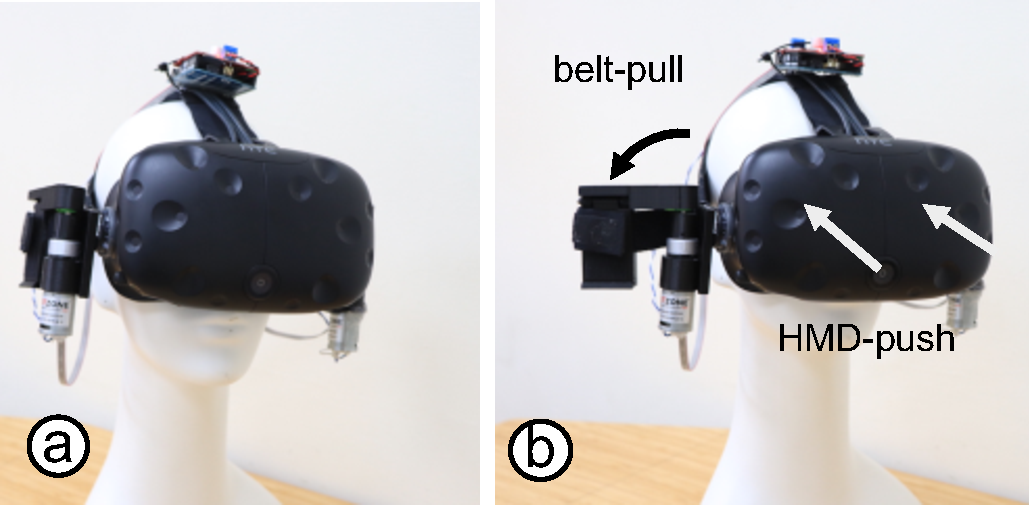
\includegraphics[width=1\textwidth]{figures/FacePush.pdf}
        \end{tabular}
        \captionof{figure}{(a) FacePush presents a pulley system incorporated with HMD providing pressure on face. (b) Our system pulls the belts of the HMD to generate discrete/continuous and weak/strong pressure stimuli to enhance}
        \label{fig:FacePush Intro}
    \end{center}
\end{figure}

Simulated haptics is a key component to enhance immersion in virtual environments. Prior research has proposed various mechanisms to generate different modes of haptic feedback. While many were deployed on limbs, e.g., through wearable interfaces \cite{Impacto} or handheld controllers \cite{normalTouch, hapticLink}, recent research has started to explore simulating haptics directly through Head-Mounted Displays (HMDs),  such as the introduction of thermal \cite{ThermoVR, Ambiotherm}, vibrotactile \cite{HapticHead} and force \cite{GyroVR, HangerOVER} feedback on users' head or face.

\section{FacePush }

In line with such efforts, we present \textit{FacePush}, an HMD integrated with a pulley system that can manipulate the HMD in order to enable pressure to be applied upon the user's head resulting in a normal force on the user's face. The mechanism of FacePush is achieved by a shifting torque provided by the two motors to a facial normal force (Figure \ref{fig:FacePush Intro}(a-b)). By controlling the angles of the motors, FacePush can generate normal forces with varying strengths. 

\begin{figure}[hp]
    \begin{center}
        \begin{tabular}{@{\hspace{0.1cm}}c}
           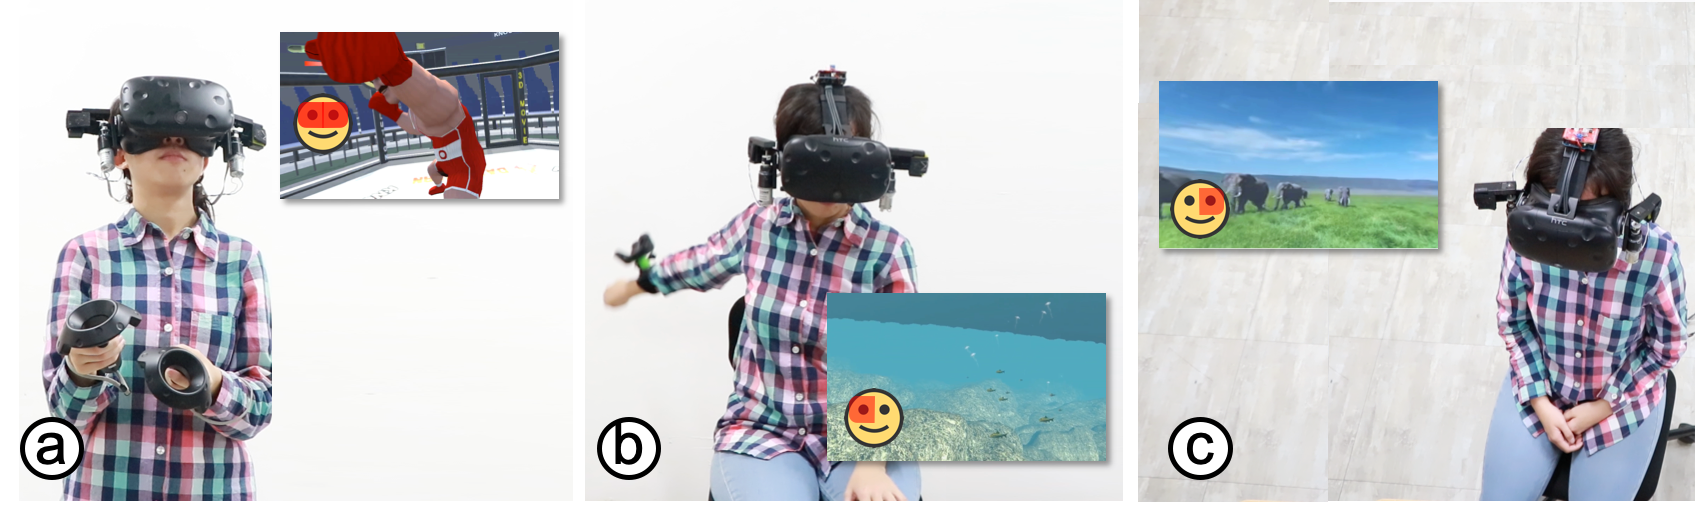
\includegraphics[width=1\textwidth]{figures/3Applications.png}
        \end{tabular}
        \captionof{figure}{(a) Boxing (b) Diving and (c) Attention guidance experiences in virtual environments. In (a)(b)(c), the face icons indicate the displayed force on face.}
        \label{fig:3Applicaions Intro}
    \end{center}
\end{figure}

FacePush allows an improvement in the sense of presence for example applications such as boxing (Figure \ref{fig:3Applicaions Intro}(a)) and underwater swimming (Figure \ref{fig:3Applicaions Intro}(b)). We also use normal force as a directional cue for direction guidance in 360 degree videos (Figure  \ref{fig:3Applicaions Intro}(c)).



\section{Contribution }

As such, FacePush offer three main contributions, namely: (1) an HMD integrated with a pulley system to render the haptic sensations via normal force acting on a user's face; (2) studies determining ADT and JND which inform effective design of noticeable and discernible normal force, along with ratings of user comfort; and (3) three applications which demonstrate use of discrete and continuous normal force that enhance user experience and offer a means to convey direction guidance.
\chapter{Related Work} \label{chapter:related_work}
In this section, we review related work on haptic output upon the face and examine previous works that use normal force to achieve haptic feedback.

\section{Haptic interaction in VR}
Simulated haptics is a key component to enhance immersion in virtual environments. Haptic interaction in VR has been extensively explored. Some works focused on installing the device on the limbs to generate partial haptic feedback for improving the realism in the virtual world, while others use large-scale device throughout the body to enhance feedback on immersive experiences.

\begin{figure}[h]
    \begin{center}
        \begin{tabular}{@{\hspace{0.1cm}}c}
           \includegraphics[width=1\textwidth]{figures/Hand_RelatedWork.pdf}
        \end{tabular}
        \captionof{figure}{(a) Haptic Revolver (b) 
Grabity}
        \label{fig:Hand_RelatedWork}
    \end{center}
\end{figure}

Most of the devices on the hand generating tactile feedback are mounted on the finger or palm. Whitmire et al. \cite{hapticrevolver} presented Haptic Revolver, a handheld VR controller that renders fingertip haptics when interacting with virtual surfaces. Grabity \cite{Grabity}, a wearable haptic device, demonstrated simulating grip forces and weight for grasping virtual objects in the virtual environment. In addition to tactile feedback for texture and precise finger manipulation, some other works focused on the bigger human motion on the arm and feet. Impacto \cite{Impacto} decomposed a series of the haptic sensation on limbs into tactile triggering and muscle contraction, using electrical muscle stimulation (EMS) embedded design to enhance the haptic feedback on limbs in VR. Lopes et al. \cite{VRwalls} actuated the user's shoulder, arm, and wrist muscles with EMS, creating a counter force that pulls the user's arm backward to add haptics to walls and other heavy objects in the virtual environment. Level-ups \cite{Level-up} showed a foot-mounted device with computer-controlled stilts that allows VR users to experience walking up and down steps.


\begin{figure}[h]
    \begin{center}
        \begin{tabular}{@{\hspace{0.1cm}}c}
           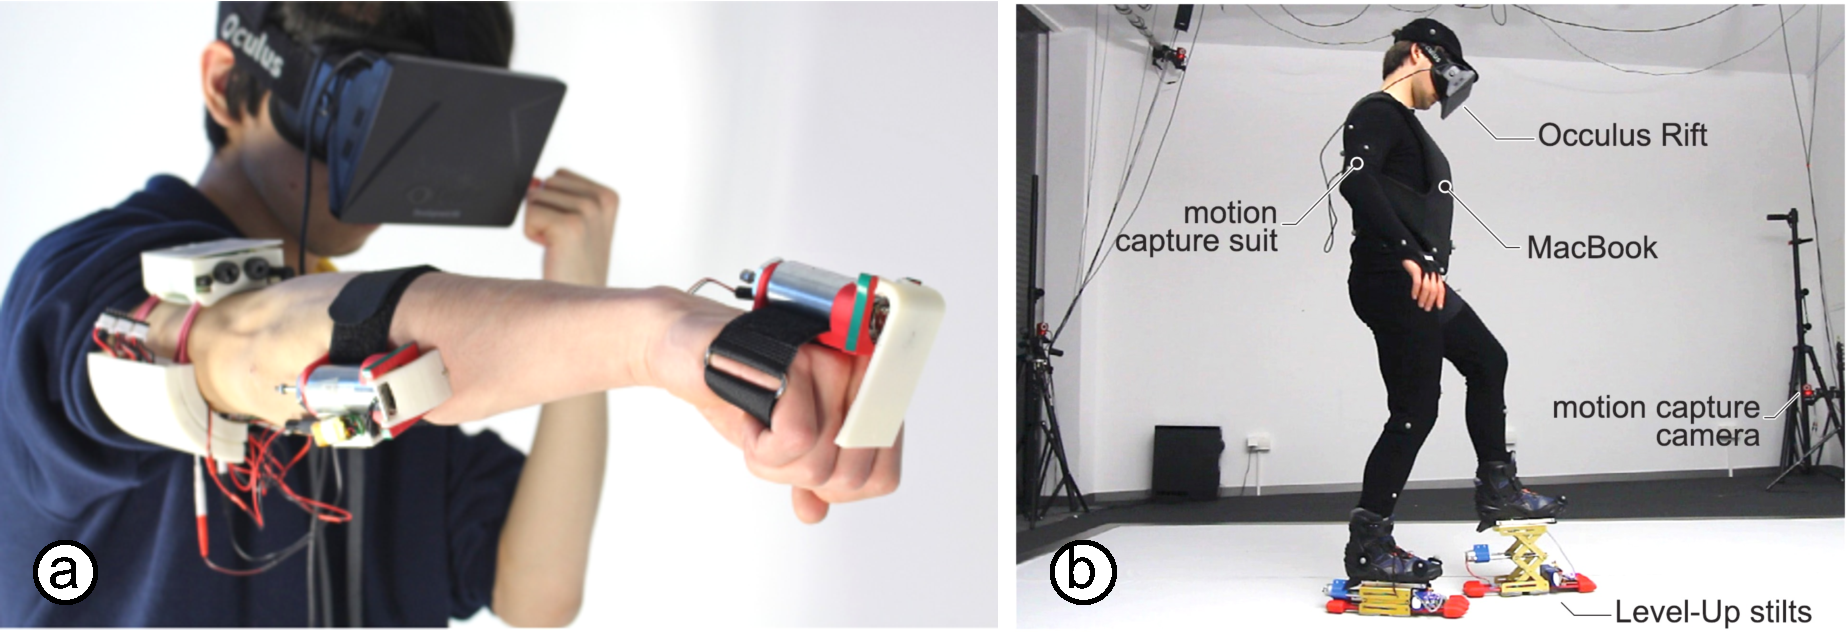
\includegraphics[width=1\textwidth]{figures/Force_RelatedWork.pdf}
        \end{tabular}
        \captionof{figure}{(a) Impacto (b) 
Levels-Up}
        \label{fig:Force_RelatedWork}
    \end{center}
\end{figure}

Apart from enhancing actuators on the human body, daily necessities have been adopted to enhance immersion. Gugenheimer et al. \cite{SwiVRChair} presented  SwiVRChair, which nudges users' orientation in 360-degree storytelling scenarios through a motorized swivel chair. Haptic Bed \cite{HapticBed} demonstrated a bed-style haptic display that provides weight sensation to the wide area of the user's body. Total resistance exercise (TRX) and elastic belts produce suspension force, enriching haptic force feedback. Hong et al. \cite{Wakeboarding} implemented Wakeboarding, in which the player riding a balance board in the reality skis on a meandering river in VR. The movement of the user was achieved by sustaining the weight and balance with the support of the suspension kit. Jain et al. \cite{Amphibian} created Amphibian, a simulator to simulate a wider variety of sensations experienced underwater through elastic band. Human-actuator also provides the user an immersive experience \cite{HapticTurk, TurkDeck}. Haptic Turk replaced motors and mechanical components with humans, a different approach to motion platforms that is light and mobile. TurkDeck produced the haptic sensation using props i.e. when users touch or manipulate an object in the virtual world, they simultaneously also touch or manipulate a corresponding object in the physical world. 


\section{Haptic Output on HMDs }
Although previous research has broadly explored various mechanisms generating different modes of haptic feedback in VR, many involved feedback as perceived via the limbs of the human body mainly achieved via handheld devices or wearable interfaces. Such haptic implementations on the limbs convey the concept of manipulating the virtual world directly. However, the human head is anatomically in charge of navigating and spatial awareness and can also be well-utilized to enhance a sense of immersion during VR encounters. The mere action of channeling haptic feedback directly through an HMDs acts as a directional information-containing medium and its design is also challenging due to the fact that every device has to be integrated into an overarching system.

\begin{figure}[h]
    \begin{center}
        \begin{tabular}{@{\hspace{0.1cm}}c}
           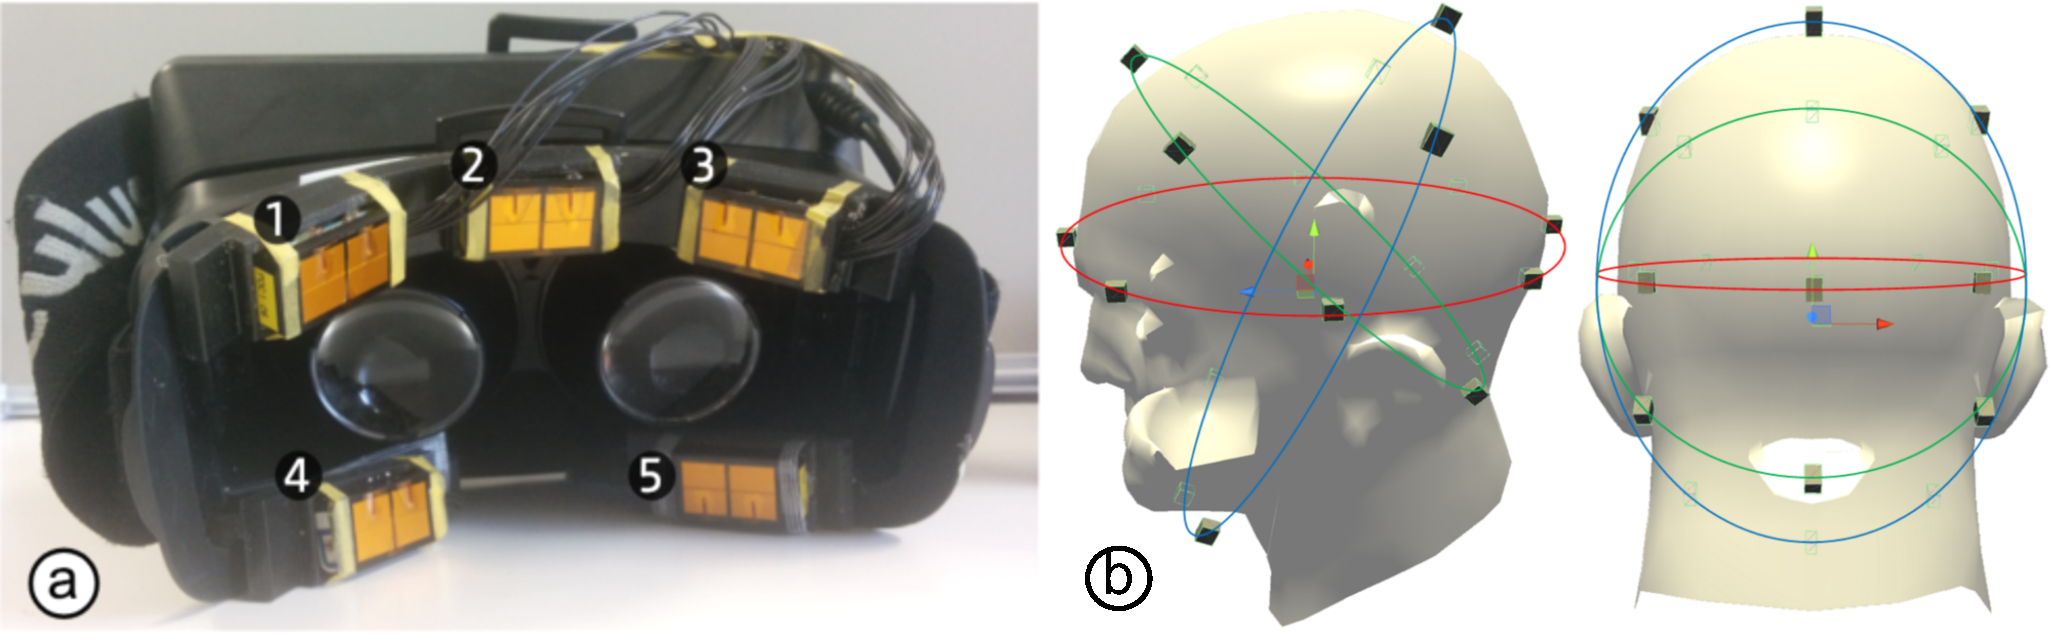
\includegraphics[width=1\textwidth]		{figures/Head_RelatedWork.pdf}
        \end{tabular}
        \captionof{figure}{(a) ThermoVR (b) 
HapticHead}
        \label{fig:Head_RelatedWork}
    \end{center}
\end{figure}

In prior research works vibrotactile feedback is implemented via HMDs that transforms haptic output into directional and guidance cues in a 3D space \cite{VibGuide, HapticHead, Vibroplay}. Consequently a vibrotactile device can be installed inside the contact region of an HMD directly and exploited as a navigation indicator \cite{VibGuide}. HapticHead \cite{HapticHead} distributes multiple vibrotactile actuators in three concentric ellipses around the head to provide intuitive haptic guidance. Vibroplay \cite{Vibroplay} extended the functionality of vibrotactile output in VR into a direct authoring manipulation system. In addition to vibrotactile feedback, thermal may be utilized as another haptic output component in a virtual environment. ThermoVR \cite{ThermoVR} demonstrates embedding of five thermal modules via HMD, which produce hot and cold haptic feedback. The different locations of thermal stimuli had been used prior as a directional cue in exploring the virtual world. Ranasinghe, et al., \cite{Ambiotherm} implements Ambiotherm, a multimodal interface including temperature modules attached to the neck and wind modules attached to the HMD allowing users to experience the sensation of wind on her/his face and the feeling of heat on the skin. 

\begin{figure}[h]
    \begin{center}
        \begin{tabular}{@{\hspace{0.1cm}}c}
           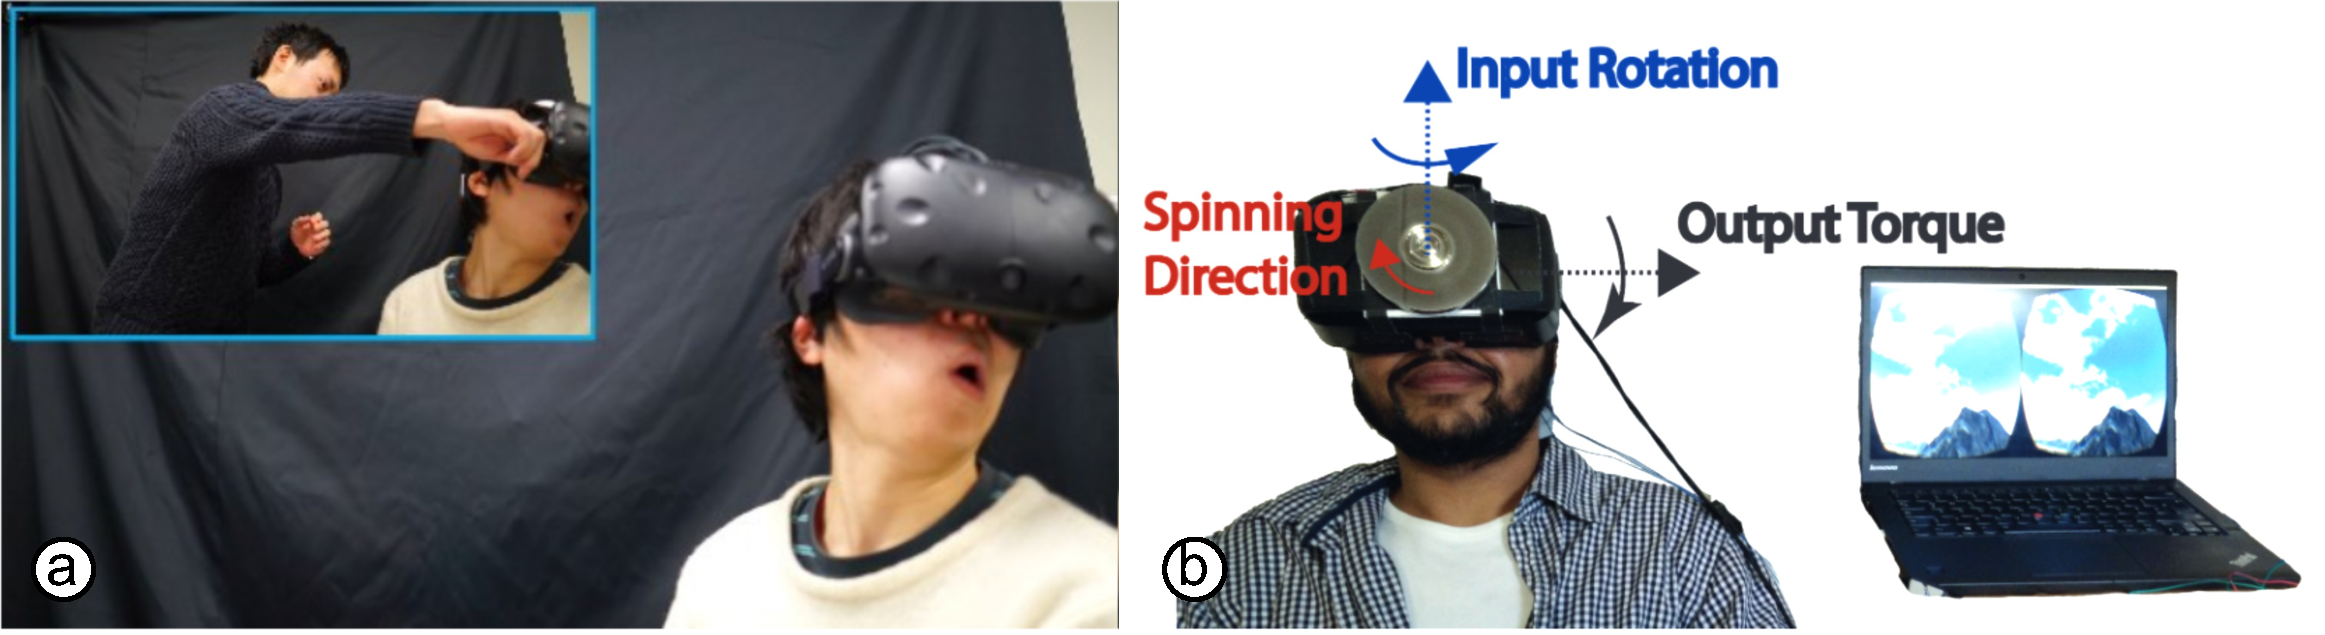
\includegraphics[width=1\textwidth]		{figures/HeadForce_RelatedWork.pdf}
        \end{tabular}
        \captionof{figure}{(a) HangerOVER (b) 
GyroVR}
        \label{fig:HeadForce_RelatedWork}
    \end{center}
\end{figure}

Other works focus on simulating head movements through force feedback. GyroVR \cite{GyroVR} contains a gyroscope attached to the HMD generating tangential force, which provides a feeling of inertia when conveying fast motion or an altered environment in VR. Sato, et al., \cite{hangerreflex09} introduce a phenomenon called “Hanger Reflex” and utilize its mechanism to implement a head rotation interface through a hanger. Kon, et al. \cite{hangerreflex16} extended the hanger reflex interface into a wearable haptic device, which can be installed on the waist. HangerOver \cite{HangerOVER} demonstrates a hanger reflex system incorporated into the HMD, allowing simulation of being pushed or punched enhancing rotation movement in a virtual environment \cite{HangerOVER}. Aoyama, et al., \cite{GVS} present the Electrode that can also simulate virtual head movement which uses galvanic vestibular stimulation (GVS) to induce a feeling of directional virtual head motion through four electrodes. Finally, GVS Ride \cite{GVSRIDE} demonstrates tri-directional acceleration through a four-pole GVS mounted with HMD.

\section{Normal Force as a Haptic Output }

\begin{figure}[h]
    \begin{center}
        \begin{tabular}{@{\hspace{0.1cm}}c}
           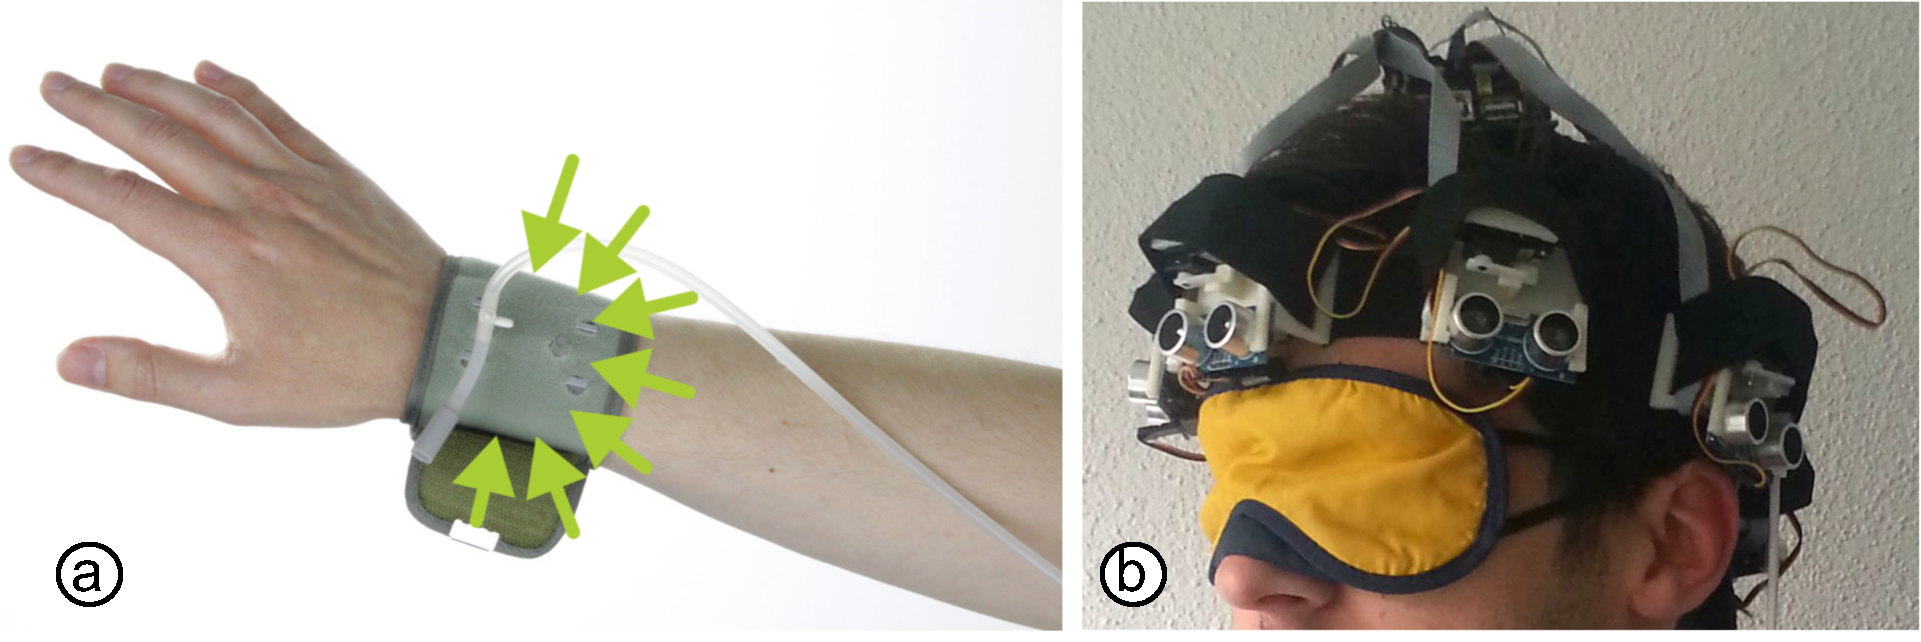
\includegraphics[width=1\textwidth]		{figures/NormalForce_RelatedWork1.pdf}
        \end{tabular}
        \captionof{figure}{(a) Squeezeback (b) 
ProximityHat}
        \label{fig:NormalForce_RelatedWork1}
    \end{center}
\end{figure}

Human beings experience normal force on a certain skin surface as a sensation of pressure through mechanoreceptors. Squeezeback \cite{Squeezback} presents the use of pneumatic actuation and inflatable straps to create compression stimulus on the wrist for notification. HapticClench \cite{HapticClench} demonstrates a squeezing sensation with a shape memory alloy on the wrist. Delazio, et al., \cite{forceJacket} presents Force Jacket, a wearable jacket attached with pneumatically actuated airbags and force sensors that provide precisely directed force and high frequency vibrations to the upper body. Berning, et al., \cite{ProximityHat} implement ProximityHat which consists of wearable pressure actuators placed around the head to convey spatial information. Based on these previous works just mentioned, we deploy the spatial information concept through FacePush which generates normal force feedback on a horizontal axis of the face via the HMD.

\begin{figure}[h]
    \begin{center}
        \begin{tabular}{@{\hspace{0.1cm}}c}
           \includegraphics[width=1\textwidth]		{figures/NormalForce_RelatedWork2.pdf}
        \end{tabular}
        \captionof{figure}{(a) HapticClench (b) 
Force Jacket}
        \label{fig:NormalForce_RelatedWork2}
    \end{center}
\end{figure}

\chapter{FacePush System} \label{chapter:system}
To render normal force feedback on the face, FacePush utilizes the original components of a Vive HMD\footnote{\url{https://www.vive.com/tw/}}, including face foam and belt. Just hereafter, we describe the hardware and software of our system as well as the mapping of motor rotations to apply pressure to the face.

\section{The Mechanical Design of FacePush }

\begin{figure}[h]
\begin{center}
    \begin{tabular}{@{\hspace{0.1cm}}c}
    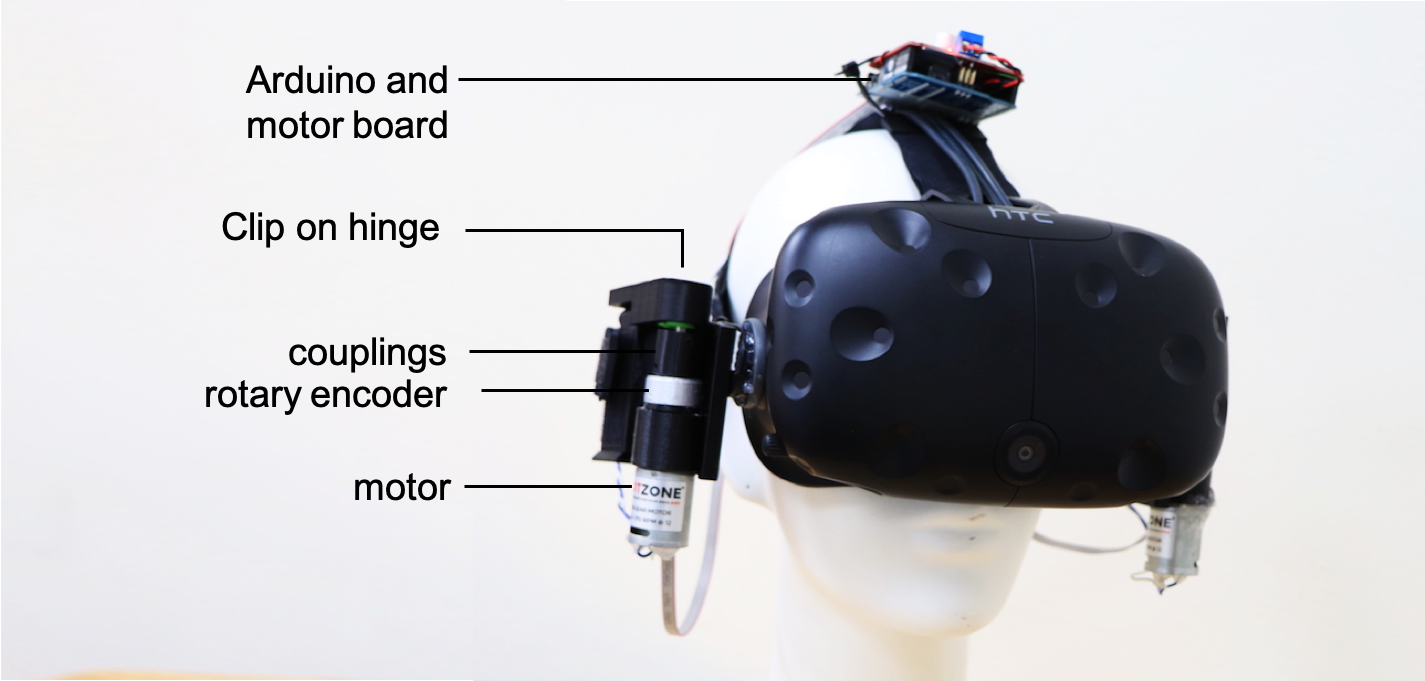
\includegraphics[width=1\textwidth]{figures/FrontView.png}
    \end{tabular}
    \caption{A front view of the FacePush system.}
    \label{fig:FrontView}
    \end{center}
\end{figure}

We considered the haptic feedback acting on the face as an embedded component installed in the HMD itself. The contact region of the foam in the HMD is a natural haptic space and the belt of the HMD, which is similar to a goggle strap,can provide  enough  constraint  to  tighten  the  headset. By tightening this belt, the user will experience a force like the face being pushed forward as pressure acts upon the face.

% In this case, 
We tested several different specifications of DC motors. Based on our experience and through design iterations, we suggest that the torque should exceed 2 N-m to provide enough power to pull the belt. However, their weight and size should be less than 100g, otherwise, the weight of the motor will restrict the movement of the user and reduce usability. We chose the 170 RPM Econ Metal Gearmotor, weighing at 92.1g, as the force actuators in our system. These motors are driven through an external motor driver (VNH2SP30-E) by a pulse width modulation (PWM) signal, with a power supply rated at 12V, 3.8A. In addition, the motors are controlled by a proportional-integral-derivative (PID) controller to ensure high positional accuracy. The PID loop iterates on an Arduino UNO board interfaced with a PC using a USB serial connection running at a 9600 baudrate.

\subsection{Torque Generators }

\begin{figure}[h]
\begin{center}
    \begin{tabular}{@{\hspace{0.1cm}}c}
        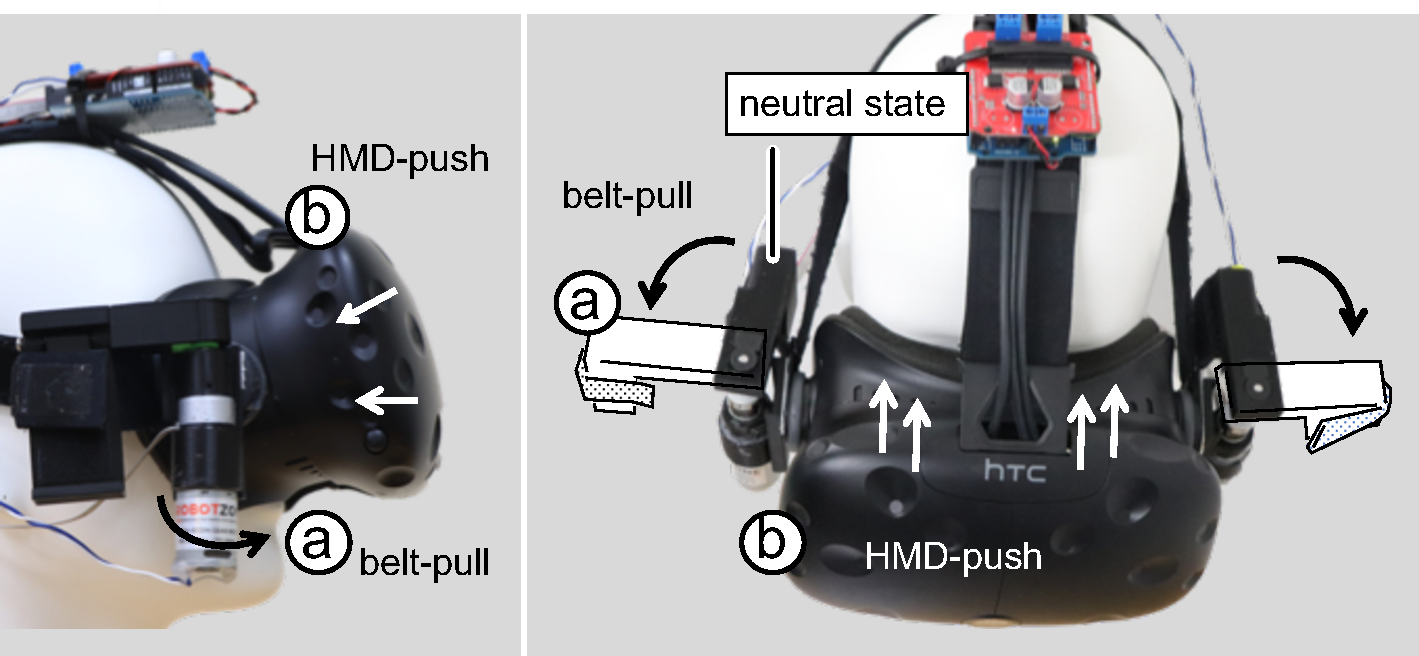
\includegraphics[width=1\linewidth]{figures/mechanical-design3}
    \end{tabular}
    \caption{Each motor connecting a belt via a torque generator allows (a) translate a belt-pull into (b) a HMD-push, resulting in a normal force on face.}
    \label{fig:mechanical_design}
 \end{center}
\end{figure}

As shown in Figure \ref{fig:FrontView}, two 3D-printed components are driven by the motors which were designed to fulfill these needs. These 3D-printed components, or torque generating components, are connected to the motor shaft through the coupling and they have a clip-on-hinge structure to grip the belt of the HMD and fasten them further when they are turned by the motor. (Hereafter these components will be referred to as ``torque generators'' for brevity.) Each motor has a rotary encoder attached to the shaft for recording its current position. The torque generators are attached to the left and right sides of the HMD. The clip structure and Velcro fasteners allow users to adjust the initial tautness of the belt (Figure \ref{fig:assemblyandsystem} a-c). 

\begin{figure}[b]
\begin{center}
    \begin{tabular}{@{\hspace{0.1cm}}c}
    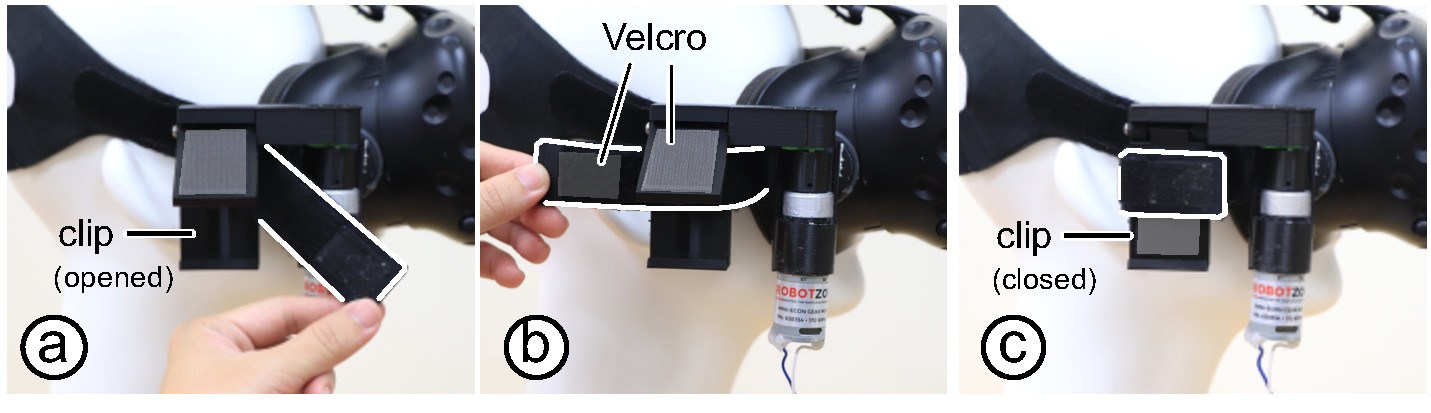
\includegraphics[width=1\textwidth]{figures/AssemblySystem.pdf}
    \end{tabular}
    \caption{(a)(b)(c) Assembly of FacePush on the HMD. The belt and the Velcro fasteners are touched for clarity.}
    \label{fig:assemblyandsystem}
    \end{center}
\end{figure}

Our torque generators transfer the torque generated by the motor shaft into a force exerted on the face. As displayed in Figure \ref{fig:mechanical_design}, we define the neutral state of FacePush as being when the torque generators are positioned parallel to the direction of a user facing forward. This is also the initial state of each ``push'' or application of force, so that each push has a reference point.

We assign the angle of the torque generators to 0 degrees. Both components can rotate at most 170 degrees, moving clockwise to the left and counterclockwise to the right. When the torque generators leave their neutral state, the belt is pulled tight and the user's face is forced forward. This force makes the entire HMD tighter and the user will experience a normal force acting on her/his face. 

\subsection{Two States of FacePush }

According to the position of the torque generators, we define two states for the behavior of FacePush. First one is \textit{Neutral State} (Figure \ref{fig:2_States} a). The neutral state represents torque generating components are positioned parallel to the direction of a user facing forward. At this moment, The rotate angle is 0 and there is no normal force exerted on the user's face. When the motor rotates, it drives the 3D-printed components and the belt is pulled. The belt-pull leads to a HMD-push resulting a normal force exerted on the user's face. We define this situation as \textit{Push State} (Figure \ref{fig:2_States} b). It represents the torque generating component is rotated and translates a belt-pull into a HMD push. At this moment, we can assign the angle to generate different magnitude of normal force during the Push State. Then, based on the behavior of the normal force, we design two different types of stimuli.

\begin{figure}[h]
\begin{center}
    \begin{tabular}{@{\hspace{0.1cm}}c}
    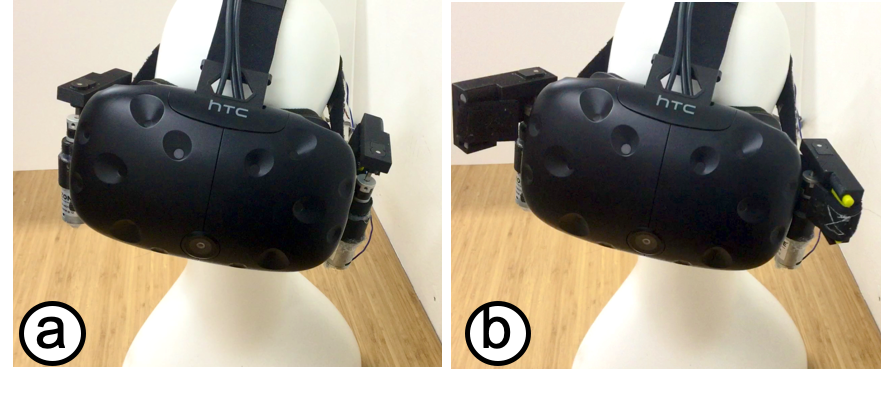
\includegraphics[width=1\textwidth]{figures/2_StatesOfFacePush.png}
    \end{tabular}
    \caption{(a)Neutral State: There is no normal force generated, when the rotate angle is 0. (b)Push State: Generates a variety of magnitude of normal force with different angle}
    \label{fig:2_States}
    \end{center}
\end{figure}

\subsection{Two Types of Stimuli}

FacePush can generate either a weak, or a strong, stimulus based on the pressure intensity at different angles. We define two types of stimuli according to their implementation in our example applications. 1) \textit{Discrete stimulus}: It is an impulse representing a short duration of contact. The duration is 0.5 seconds. Thus its impulse increases and decreases instantly; this is utilized in our boxing application(Figure \ref{fig:2_Stimuli} a). 2) \textit{Continuous stimuli}: The duration covers the whole application, but the intensity is different among users. We use these stimuli depends on the scenario of applications. In the virtual diving example application(Figure \ref{fig:2_Stimuli} b), the simulated water current is generated according to the displacement of the player every three frames during rendering VR scene. The stimuli provided by our system allow for a variety of haptic feedback on the face for VR applications.

\begin{figure}[h]
\begin{center}
    \begin{tabular}{@{\hspace{0.1cm}}c}
    \includegraphics[width=1\textwidth]{figures/BoxingAndDiving.pdf}
    \end{tabular}
    \caption{(a)Discrete stimulus: An impulse representing a short duration of contact. (b)Continuous stimuli: The duration covers the whole application, but the intensity is different among users.}
    \label{fig:2_Stimuli}
    \end{center}
\end{figure}

\section{Mapping Rotated Angle into Pressure on Face}

\begin{figure}[h]
    \begin{center}
        \begin{tabular}{@{\hspace{0.1cm}}c}
            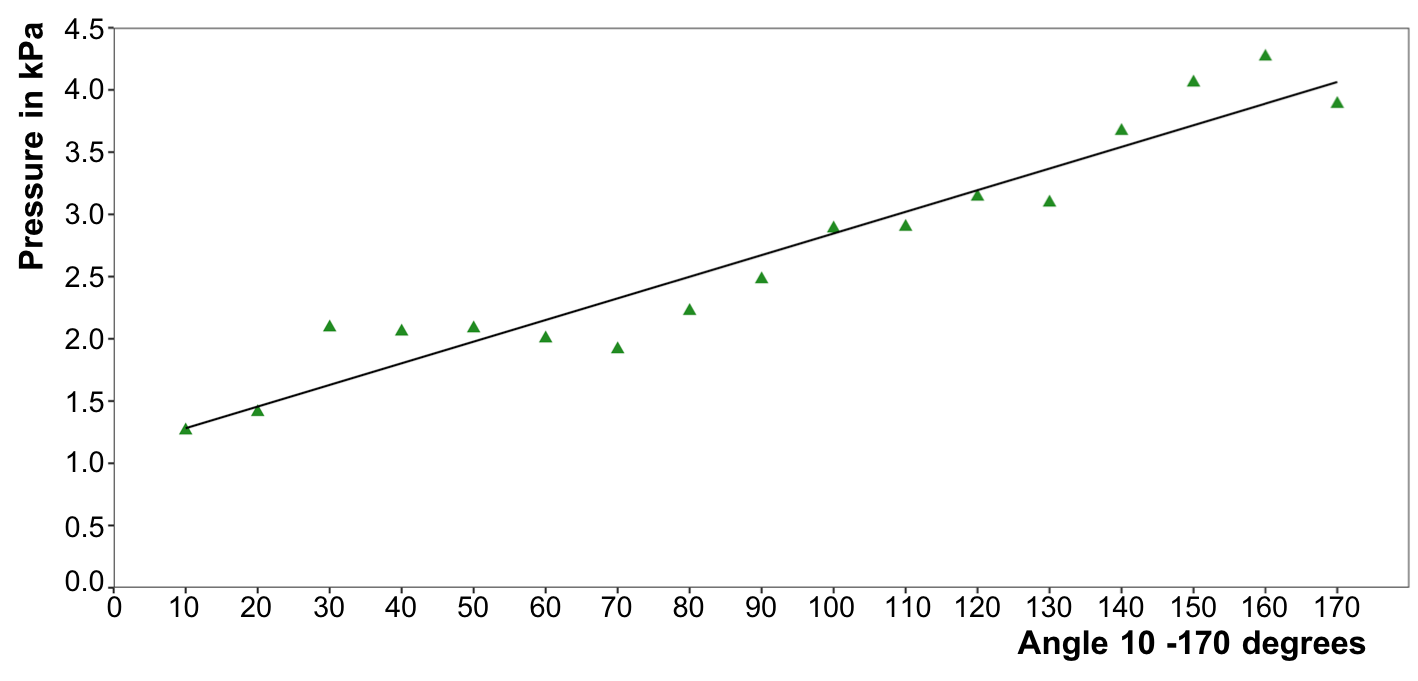
\includegraphics[width=1\linewidth]{figures/a2p}
        \end{tabular}
        \caption{Angle to pressure mapping.}
        \label{fig:angle_to_pressure}
    \end{center}
\end{figure}

As FacePush can make its torque generators rotate to a specific angle, we were interested in how much pressure is provided on the face by FacePush within their rotational range of 0 to 170 degrees. We set up a force sensing resistor to measure the relationship between the pressure exerted against the different rotating angles of the torque generators. Five FlexiForce Pressure Sensors 1 lb\footnote{\url{https://www.tekscan.com/flexiforce-load-force-sensors-and-systems}} were attached to a one-to-one ratio mannequin head. The attached positions were cheekbone (left and right), the upper region of the tail of eyebrow (left and right), and forehead. The torque generators started from their neutral state and rotated through 10 to 170 degrees in steps of 10 degrees each. The motors were driven at their full speed (with a PWM value of 255). Data from the sensor at the forehead were removed since it was discovered that the pressure was primarily distributed on the both sides of the mannequin's face. The values from the remaining four sensors were averaged and a linear equation derived for the mapping between motor angles and the derived pressures as shown in Figure \ref{fig:angle_to_pressure}: (y = 1.108 + .017x, R$^2 >$ 0.9). The measurement obtained here is the pressure on a single sensor, which is proportional to the total force exerted on the user's face. The total force can be calculated by multiplying the pressure by the contact area of the facial interface of the HMD. These results confirm the relationship between the angle and the pressure exerted on the face.
\chapter{Example Applications} \label{chapter:interaction_techniques}
We have determined two levels of normal force at 2.7 kPa, and 3.375 kPa, referred to as light and strong forces, which are noticeable and discernible according to our studies of Absolute Detection Threshold (ADT) and Discrimination Threshold (JND). Based on FacePush, we introduce three VR applications embedded with the normal force haptic feedback on the face. In the first and second applications, the interaction provides discrete and continuous normal force depending on the duration of haptic feedback acting on a user's face. For the third, FacePush provides continuous normal force which are used to guide users toward a region of interest (ROI) when exploring 360 degree videos. 

\section{Boxing: Discrete Force on Face OK}

FacePush can provide discrete normal forces simulating immediate pressure acting on the face. This discrete haptic feedback was given a trial run in a virtual boxing scenario. Therein the user stays in a standing pose to experience our boxing application and the avatar of an opponent appears in front of the user in virtual reality.

As the application begins to run the play scenario, the opponent throws punches consecutively. As each punch hits the left, right, and middle of the user's virtual face, FacePush engages the left motor, right motor, and both motors, respectively. In addition to the area hit, distinguishable normal force stimuli are provided by FacePush that also simulate the varied strengths of the punches. (Figure \ref{fig:boxing}) displays examples of the force of the punches landed. The opponent is programmed to randomly throw jabs, straight blows or hooks from left or right. A jab is fast and light. A straight punch is a longer punch of a medium strength. A hook is a curvy punch with great strength. We mapped the strength of each punch onto the two levels of normal force provided by FacePush. The area hit and the strength of a punch are calculated in real time from the opponents boxing motions. 
%A health bar was displayed to remind the user of her/his remaining health points. 

An emoji is displayed on the lower-left area of the user's field of view (FOV) which area for where each hit is landed. Users experience different kinds of punches and they also suffer different degrees of virtual damage. At the moment of being hit, the camera view of the user shakes instantly as a visual stimulus, and the motors will rotate according to the strength and area hit simultaneously providing haptic feedback on the face.

\begin{figure}[h]
    \begin{center}
        \begin{tabular}{@{\hspace{0.1cm}}c}
            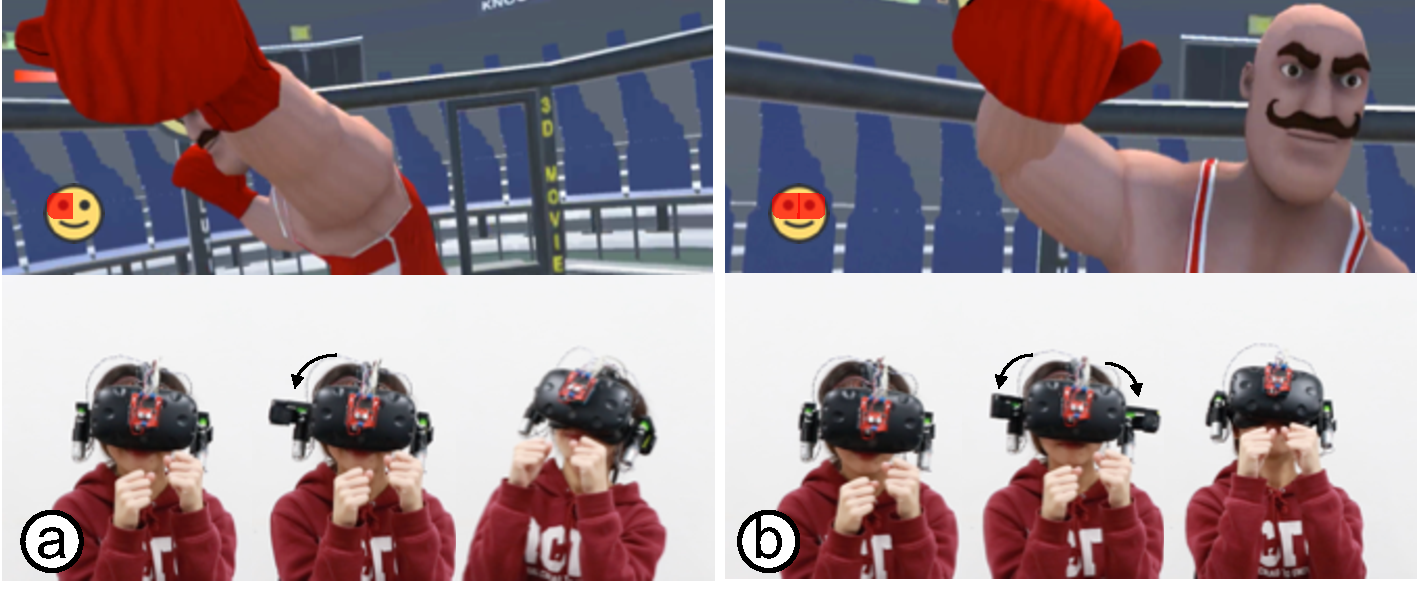
\includegraphics[width=1\linewidth]{figures/boxing2}
        \end{tabular}
        \caption{Boxing experience: a punch hit at the left and middle areas of the user face triggers the left and both motors respectively. (The mark on the cloth was masked for blind review.)}
        \label{fig:boxing}
    \end{center}
\end{figure}

\section{Diving: Continuous and Discrete Normal Force OK}

Continuous normal force simulates pressure acting on a face over a time span, e.g., the flow of water acting on the face when swimming creates a continuous pressure on the face. In this virtual experience, we created a diving scenario to demonstrate the haptic feedback of the pressure of water flowing across the face. 

The user is seated in a chair and wears wrist straps on both forearms each attached to a Vive tracker. The Vive trackers record the orbits of the hands' positions. When a user makes actions with the hand similar to say a breaststroke for example, the orbits of the two trackers are used to calculate the direction of motion and speed of the user virtually. A left-arm stroke leads to a right turn and a right-arm stroke leads to a left turn. If the user makes arm strokes with both hands, she/he will move forward (Figure \ref{fig:diving-fishshark}(a-b)). Meanwhile, a corresponding normal force is generated to simulate the water flowing across the face. For example, while swimming to the right, the right motor will give force to the right side of the user's face. If the user is moving forward, both motors start turning to a specific angle and keep holding the belt during the advancing term. Depending on the speeds of motion, we set the force to increase up to light or medium level and then fade out the force.

In the diving scenario, we also present two underwater haptic experiences, as displayed in (Figure \ref{fig:diving-fishshark}(c-d)). Users can experience passing through a school of fish.
A user's face will receive a normal force alternating on their left and right sides. FacePush simulates the experience with light force. In the second experience, a shark swims toward the user and then turns away at close range; the current from this virtual encounter exerts a strong normal force on the user's face.

\begin{figure}[h]
    \begin{center}
        \begin{tabular}{@{\hspace{0.1cm}}c}
            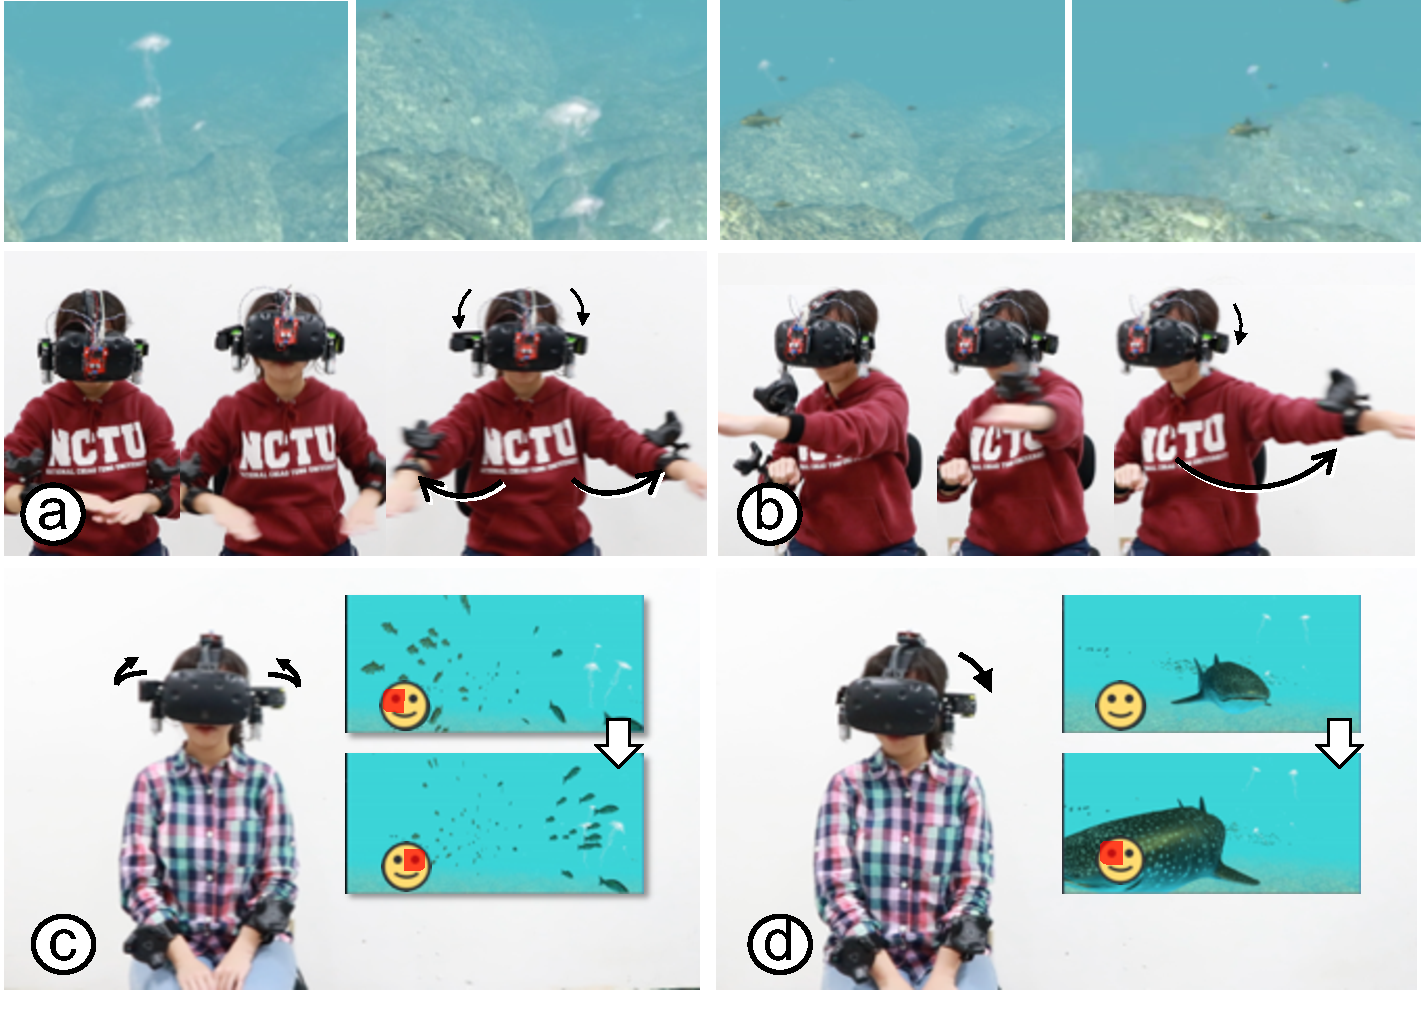
\includegraphics[width=1\linewidth]{figures/diving-fishshark2}
        \end{tabular}
        \caption{Diving experience: the user advances underwater with arm strokes of both hands, and turn left with right-arm strokes.  (The mark on the cloth was masked for blind review.)}
        \label{fig:diving-fishshark}
    \end{center}
\end{figure}

\section{Attention Guidance: Continuous Normal Force OK}

The users of 360 degree videos sometime suffer from missing regions of interests (ROI) in any given video clip. In this implementation of FacePush, we mapped the normal forces generated by the left and right torque generators onto a directional cue of yaw axis in 360 degree videos. 

%Lin et al. \cite{} proposed using a picture-in-picture technique and show which side should the user rotate to 
Here, the normal force generated by FacePush exerted on the user's face is used to prompt targets for the attention of the viewer in 360 degree videos. That is, when a target is beyond the user's field of view on the left side of the user, FacePush engages the left motor to indicate the target's direction. The intensity of normal force is determined based on the rotational angle to bring the target into the FOV. When the angle is less than 30 degrees, a light force is applied; otherwise, a medium force is applied. Once the target appears in the user's field of view (FOV), the force disappears. This trial implementation utilizes a sample wildlife 360 degree video (Figure \ref{fig:attention-guidance}). The user looks for animals on a plain, and FacePush prompts the user to locate where there the animals are.

\begin{figure}[h]
    \begin{center}
        \begin{tabular}{@{\hspace{0.1cm}}c}
            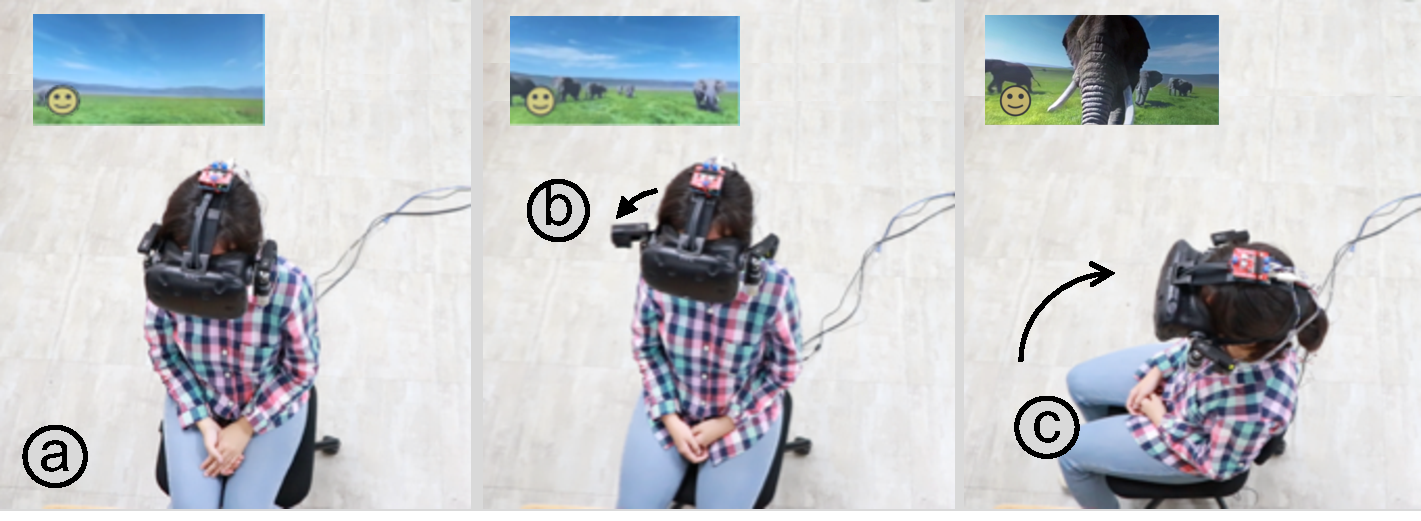
\includegraphics[width=1\linewidth]{figures/attention-guidance2}
        \end{tabular}
        \caption{Attention Guidance: left or right-sided normal force on face guides users to search toward left or right respectively.}
        \label{fig:attention-guidance}
    \end{center}
\end{figure}
\chapter{User Studies} \label{chapter:evaluation}
In the user study 1, we conducted an absolute detection threshold (ADT) study and a discrimination threshold (JND) study to investigate how users perceive normal force stimuli provided by FacePush. Additionally, we collected users' subjective ratings of their comfort with respect to the normal force feedback. Based on the results of user study 1, we determined the magnitude of normal force for the boxing application and ran an experience study using the boxing scenario.


\section{User Study 1: Psychophysics of FacePush}

\subsection{Absolute Detection Threshold (ADT) OK}
To determine the minimum normal force that is provided by FacePush that users can perceive, we conducted a standard two-down, one-up staircase study \cite{Lynette2012, Leek2001}. In each trial, both torque generators started rotating from their neutral state to a specific angle simultaneously. When the torque generators achieve the target angle, they maintain exertion of normal force on the face for a brief duration then return to their neutral state. The entire trial process is 4 seconds and the interval between two consecutive trials lasts 5 seconds. The experiment starts finding threshold from the high degree (150 degrees from the neutral state) to the absolute detection threshold. When participants perceive the stimulus twice consecutively, the target degree of the torque generators is decreased by a step size. Otherwise, the target angle increases if the stimulus is not felt at least once. The step size is 12 degrees and it is divided by two for every eight trials. The average of the last five trials performed are taken as the threshold estimate. These values were determined from a pilot study in which participants needed to complete 24 trials for three reversals. Each participant presses the play button when they are ready, but only once per trial, and responds with an answer of either “Felt” or “Not Felt” after each stimulus. For each trial, the participant's response was recorded and the corresponding angle of the torque generators. Each participant performed 72 trials in total and the entire procedure took approximately one hour to complete. During this study, the participant wore earphones with pink noise. Participants received a small gratuity as compensation for their time. 

\subsection{Results OK}
Nine participants (4 females and 5 males, aged 22-26, mean age = 23.8) were recruited from our institution. The mean threshold estimate was 2.694 kilopascal (kPa) (95\% CI [2.558, 2.83]) which indicates that both torque generators must generate at least 2.694 kPa, which rotate 86 degrees from their neutral state such that a participant begins to feel the pressure on their face.

\subsection{Discrimination Threshold (JND) OK}
We are also interested in how users can distinguish a normal force stimulus exerted by FacePush. Hence, we conducted a just-noticeable difference (JND) study using the method of constant stimuli. Each participant had to respond \textit{same} or \textit{different} for each stimulus pair and each pair consisted of a base load and an offset load value. The torque generators can only rotate from 0 to 170 degrees and must rotate 86 degrees from their neutral state to reach the minimum detectable threshold. Thus the range in JND study is restricted to between 85 to 170 degrees from the neutral state of the torque generators. We use four base pressures (2.575, 2.700, 2.950, 3.450 kPa) and four offsets pressures ($\Delta$P) (0, 0.125, 0.250, 0.500 kPa) providing 16 different conditions. The base offsets increase exponentially in keeping with the JND standard. The order of conditions within the stimuli pairs is randomized and each participant must repeat two reversals, resulting in 32 trials in total. The interval, between the first stimulus and the second, is 5 seconds. After the first stimulus is given, FacePush returns to its neutral state and waits for 3 seconds then begins the second stimulus. The entire procedure during this study took about 20 minutes to complete and participants wore earphones with pink noise throughout the duration of the study. The same group of 9 participants (4 females and 5 males, aged 22-26, mean age = 23.8) that took part in our ADT study took part in this study several days later.

\subsection{Results OK}

\begin{figure}[h]
    \begin{center}
        \begin{tabular}{@{\hspace{0.1cm}}c}
            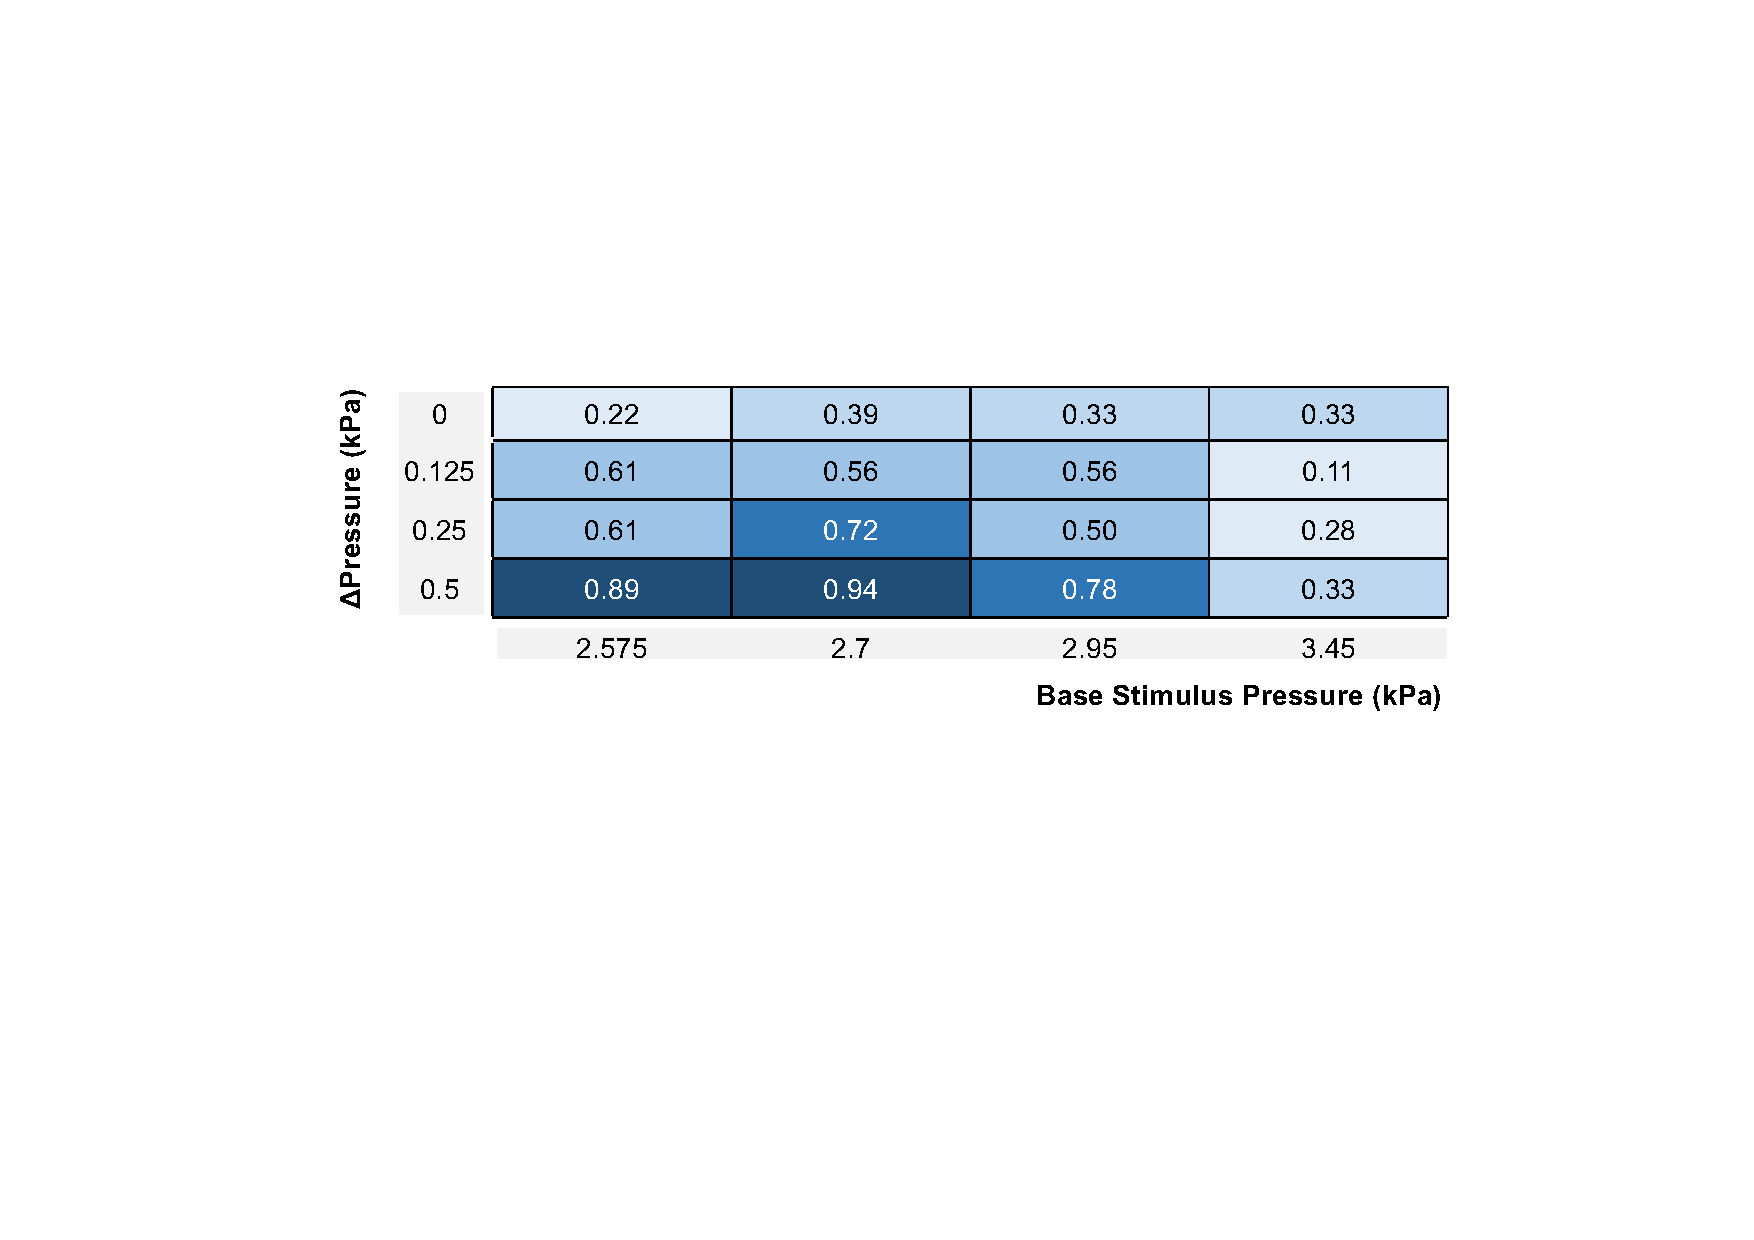
\includegraphics[width=1\linewidth]{figures/jnd}
        \end{tabular}
        \caption{Table shows the percentage of responses that judged the two stimuli as different. As baseload increases, offset needs to be higher.}
        \label{fig:jnd}
    \end{center}
\end{figure}

We define the JND as the pressure difference where 75\% of the users were able to distinguish two stimuli apart. By picking a 25\% error level, we obtained the difference where we can assume participants only confuse two different kinds of stimulus in 25\% of instances. The percentage of users who felt that a pair of stimuli are different is aggregated as a score for each base/offset pair (Figure \ref{fig:jnd}). The base rate, 2.575 and 2.700, need a $\Delta$P of 0.5 kPa so that the user can distinguish two stimuli. The other two base pressures, 2.950 and 3.450 did not perform well. We consider that these two base rates may need a greater $\Delta$P. However, not only adding more $\Delta$P for perceiving a difference from 3.450 kPa already exceeds the available range of FacePush, strong force may cause some concern in regard to comfort. Hence we selected 2.575 and 2.7 kPa as the base pressure for the comfort experiment. We determined the 75\% JND for each base value by fitting a logarithmic function to the ($\Delta$Pressure / Base Pressure) versus an aggregated percentage of the data (R$^2 = .69$) and calculating the $\Delta$P at 75\%. The 75\% JND we obtained is ($\Delta$P / Base Pressure = 0.25).

\subsection{Comfort of FacePush OK}
We investigated the subjective rating in regard to user comfort with haptic feedback while they are experiencing a normal force exerted by FacePush. In addition to comfort, we also recorded if the user felt the pressure coming from the foam of the HMD or a constraint force around her/his head. We determined six stimuli from the results in Figure \ref{fig:jnd}, two base rates (2.575 and 2.7 kPa) add 0.5 and 1 kPa, which are 2.575, 2.7, 3.075, 3.2, 3.575, and 3.7 kPa. We used a 6x6 Latin square to reduce carry-over effect. This experiment is a repeated-measures design where, each participant experiences six stimuli in six orders. 
% determined by the Latin square.
After each stimulus is given, the participant rates the comfort and indicates where the normal force is coming from. We use a 7-point Likert scale to measure comfort and the respondents may rate to one digit after the decimal (e.g., 6.1). The entire process consists of 36 trials and took about 15 minutes to complete during this study. 6 participants (2 females and 4 males, aged 22-26, mean age = 23.7) were recruited for this experiment. 

\subsection{Results OK}
The results of the comfort ratings and the percentage of feeling force coming to the face are shown in Figure \ref{fig:comfort} (Error bar shows one standard deviation). As the pressure increases, the subjective comfort decreases and the feeling of normal force is slightly turned into a constraint force around one's head. This finding informs us that the appropriate pressure stimulus exerted by FacePush should not exceed 3.5 kPa to ensure a suitable level of comfort. We chose 2.7 kPa as our criterion for pressure stimulus due to its location in the confidence interval of detectable pressure and its discernible force does not exceed the range of FacePush. This value is also acceptable as we find in the comfort study. Thus we apply 2.7 kPa in the further user experience study.

\begin{figure}[h]
    \begin{center}
        \begin{tabular}{@{\hspace{0.1cm}}c}
           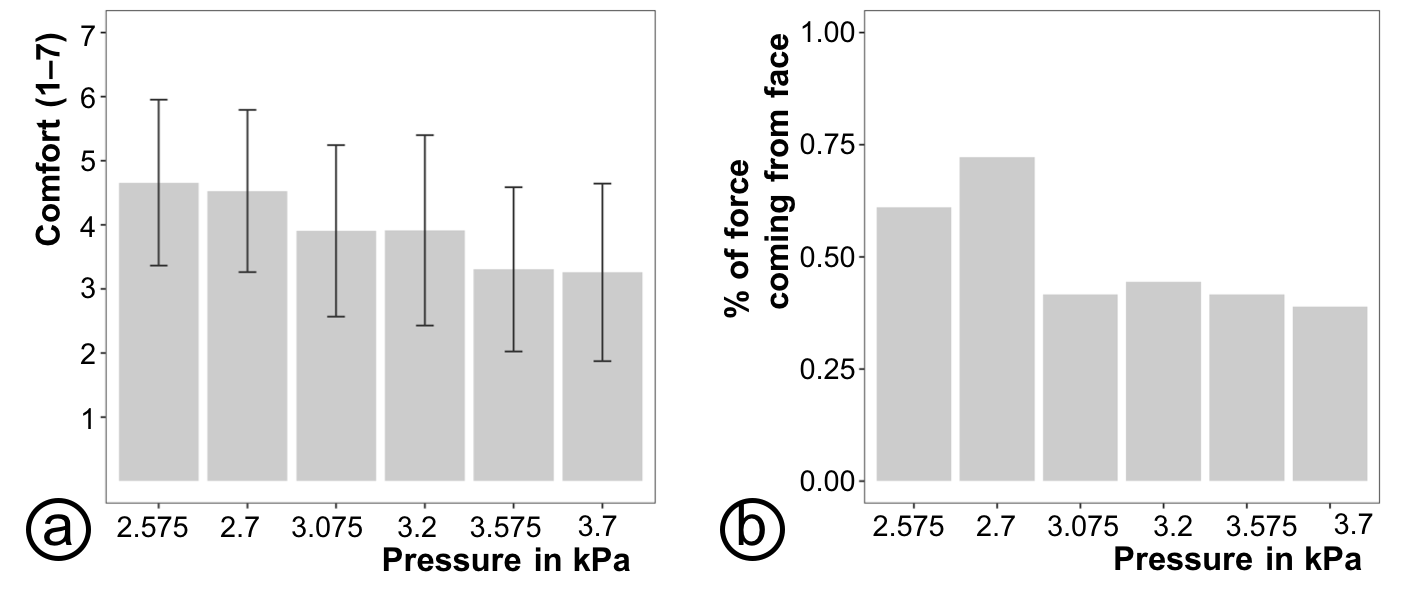
\includegraphics[width=1\linewidth]{figures/comfort}
        \end{tabular}
        \caption{(a) Comfort of each pressure (b) Judging the percentage of pressure on the face}
\label{fig:comfort}
    \end{center}
\end{figure}

\section{User Study 2: User Experience OK}
To survey the influences that FacePush can provide from the virtual world, we conducted a user study on the users of the boxing simulation. For this purpose, we immersed participants in a simplified study version of our boxing application. The participants cannot avoid being hit by the avatar. The avatar is displayed in front of the users and throws punches at the user consecutively. The level of realism and enjoyment are measured by their subjective ratings.

\subsection{Participants OK}
12 participants (7 females and 5 males, aged 21-25, mean age = 23.66) were recruited from our institution. Three of them had had no previous VR experience. Each participant received a small gratituity after completing our study.

\subsection{Experimental Design OK}
This experiment explores the effect of FacePush related to subjective ratings and head rotation. We vary the levels of FacePush as follows: 1) No-FacePush effect; the participants only wear the HMD mounted with FacePush but the FacePush device does not apply its effect. 2) FacePush with light pressure only; the intensity of each push was a constant of 2.7 kPa. 3) FacePush with heavy pressure only; the intensity of each push was a constant with 3.2 kPa. And, 4) FacePush with diverse pressure; FacePush exerts two different intensity stimuli (2.7 and 3.375 kPa) on the participants based on our results from the JND study. Each participant walks through four conditions and must assess the levels of realism and enjoyment of experiencing VR boxing.

To control the visual input across the four conditions, we display the animation of punches in accordance with a fixed order. The interval between two consecutive punches is 4 seconds long and each punch lasts approximately 0.5 seconds. The entire clip of animation for one condition runs for one minute. We asked the participants to wear earphones emitting pink noise as in the study 1.

\subsection{Procedures OK}
At the beginning of each trial, we asked the participants to maintain a standing pose and hold the Vive hand-held controllers in both hands so that they can fight against their opponents. After each condition, we asked participants to fill out a customized questionnaire to measure their experience of realism and enjoyment. The responses of questionnaire are on a 7-point Likert scale and allow for decimal responses. The order of conditions for each participant is determined by a 4x4 Latin square. Afterward, an open-ended interview to elicit general comments about the system is conducted. We also asked participants to rank their preferences of the four conditions according to their experience of realism and enjoyment respectively.

\subsection{Results OK}

\begin{figure}[h]
    \begin{center}
        \begin{tabular}{@{\hspace{0.1cm}}c}
        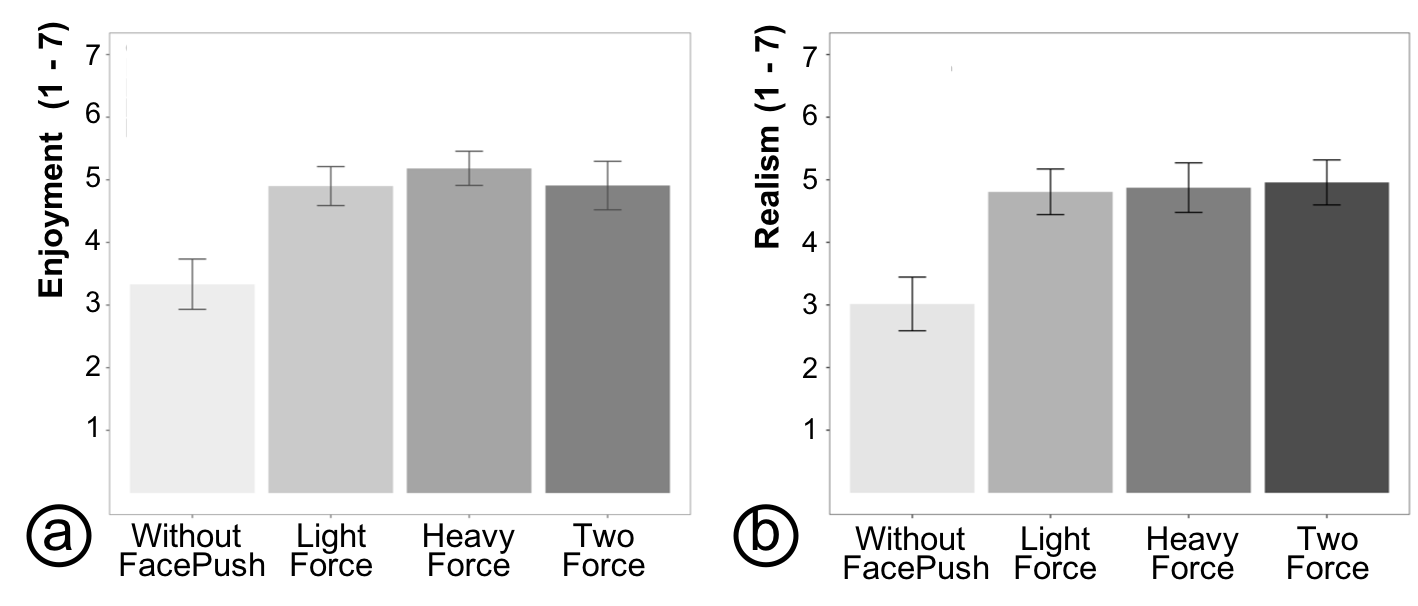
\includegraphics[width=1\linewidth]{figures/enjoymentrealism.png}
        \end{tabular}
        \caption{The subjective ratings for Enjoyment and Realism with regards to a virtual boxing application.}
        \label{fig:enjoymentrealism}
    \end{center}
\end{figure}

\subsubsection{Enjoyment}
Figure \ref{fig:enjoymentrealism} a shows the subjective ratings of enjoyment (The error-bar represents a 95\% of confidence interval). The level of No-FacePush received the lowest ratings (3.33, SD: 1.42). The ratings for the other three levels, light pressure (4.90, SD: 1.10), heavy pressure (5.18, SD: 0.965), and diverse pressure (4.91, SD: 1.37), are similar. The results of a one-way repeated measured ANOVA analysis indicates a significant difference in enjoyment ($F_{3, 33} = 22.894, p < .001$). We applied a pairwise test of means to examine the differences between level pairs. After Bonferroni correction, the level of No-FacePush is found to be significantly lower than the other three levels (light: $t_{11} = -5.585, p < .001$, heavy: $t_{11} = -5.457, p < .01$, diverse: $t_{11} = -7.021, p < .001$). The comparisons among light, heavy, and diverse levels showed no difference (light to heavy: $t_{11} = -1.982, p = 0.438$, light to diverse: $t_{11} = -0.039, p = 1$, heavy to diverse: $t_{11} = 1.104, p = 1$).

\subsubsection{Realism}
As shown in Figure \ref{fig:enjoymentrealism} b, the mean and 95\% confidence interval of subjective ratings of realism are presented. The condition of No-FacePush received the lowest rating (3.02, SD: 1.52); light pressure (4.81, SD: 1.29), heavy pressure (4.88, SD: 1.40), and diverse pressure (4.96, SD: 1.27). We conducted a one-way repeated measured ANOVA analysis and the violations to sphericity used Greenhouse-Geisser corrections to the degrees of freedom. The results indicate that the levels of FacePush show a significant difference in realism ($F_{3, 33} = 16.788, p < .001$). After Bonferroni correction, the pairwise test of means was performed and the result show that th No-FacePush level has a significant difference between light ($t_{11} = -4.579, p < .01$), heavy ($t_{11} = -4.381, p < .01$), and diverse levels ($t_{11} = -5.328, p < .01$). The comparison between light, heavy, and diverse levels showed no difference (light to heavy: $t_{11} = -0.628, p = 1$, light to diverse: $t_{11} = -0.625, p = 1$, heavy to diverse: $t_{11} = -0.279, p = 1$).

\subsection{Discussion OK}
Apart from these subjective ratings, we received user feedbacks from the interviews conducted afterward. In the interview, we asked participants to rank their preference of enjoyment and realism according to the four conditions they had experienced. Most of the participants rank the No-FacePush condition as the lowest and have a preference for the strong pressure or diverse pressure condition. This feedback corresponds to our results from inference statistics that levels of enjoyment and realism without FacePush are significantly lower than other conditions.

Users stated that, \textit{``I sometimes felt my glasses pressed while FacePush is pushing'' (P9)} and \textit{``I felt nausea during the boxing experience'' (P11)}. These uncomfortable outcomes may be caused by the distance shrinking from eyes to the lens of the HMD during pushing. This may cause the focus to change temporarily and cause nausea and blurred vision. However, we wish to stress that the participants did not explicitly report such an issue during the FacePush interaction. We think it is in part because the lens resets as soon as the short (and fast) feedback is finished during the boxing and diving applications. In the 360 video guidance trial, the continuous feedback may last longer, but the blurring effect may be ignored by users due to the only light pushes (thus short displacement) that are applied to the user's face for directional cues.

We consider that future research can address this by automating the focus adjustment via hardware solutions \cite{Konrad:2016:NOC:2858036.2858140,Optimizing.virtual.reality,Varifocal}, which exploited focus-tunable and multi-focus lenses to automatically adjust lens positions to reduce visual discomfort. Although their aim is to reduce the visual discomfort caused by vergence-accommodation conflict, the adjustment mechanism could be utilized to mitigate the lens displacement made by FacePush.In general, participants felt engaged with FacePush. For example, one participant stated that \textit{``The entire experience was very impressive, and the combination of punch feedback using FacePush was realistic.'' (P7)}. 

Our FacePush system provides only a part of the haptic feedback for a series of human sensations. Impacto \cite{Impacto} simulates boxing haptics through tactile feedback and impact movement. In future studies, FacePush's boxing experience can be enhanced with Impacto's mechanism, e.g., leading the normal force with a tactile feedback on the face. In the underwater swimming scenario, FacePush can be integrated with the thermal modules as per ThermoVR \cite{ThermoVR} to bring about sensations of coldness and distinctive current of water flowing simultaneously to enhance the user experience.


\chapter{Discussion} \label{chapter:discussion}

\section{Limitations }
FacePush has some limitations to overcome. We summarize these into three categories. First, after installing FacePush on the HMD, the weight of the whole system is easily perceived by the user. Most of the weight is caused by the motors on both sides, which may cause the HMD to slide down during the experience. Second, the motor generates some noise which can impact the user's experience. These limitations can overcome by using different actuation mechanisms, such as embedding Shape Memory Alloys into the belt, though whether that the mechanism allows sufficient speeds and strengths of forces suggested by the FacePush study requires further research. Finally, we use a pressure unit, which is proportional to the force exerted on the user's face, to represent the force in this work. Pressure is used due to the difference of facial characteristics (muscle density, etc) of the different users. In our future studies, we will address this by analyzing the different characteristics of the facial properties and facial interfaces of HMDs to quantify the actual forces.

\section{Future Work }
Currently, the haptic feedback of FacePush is focused only on the facial region of the user. In the future, we will apply FacePush's mechanism to other parts of the body, similar to HapticClench does on the wrist \cite{HapticClench} and GravityGrabber on the finger \cite{Gravity.Grabber}. In addition, we hope to combine FacePush's generated haptic feedback with other simulated facial feedback, such as tactile touch and thermal feedback.

\chapter{Thermo with Push 文字 照片} \label{chapter:Thermo with Push}

\section{Hardware Combined}

\section{Updated Applications}
\chapter{Conclusions OK} \label{chapter:conclusion}

We have introduced FacePush, a pulley system based mechanism integrated with head mounted displays to present the sensation of normal forces acting on a user's face in VR experiences. We conducted experiments to identify the absolute detection threshold and the discrimination threshold which informed an effective design for noticeable and discernible normal force and in addition, measured the comfort levels of users of FacePush. In this study a normal force was applied in three different ways and displayed in three different scenarios, namely boxing, diving, and attention guidance. According to the results of user study 2, FacePush significantly enhances the VR experience. 

\newpage
\printbibliography[heading=bibintoc,title={References}]

\end{document}